\newcommand{\delft}{
    \frametitle{
        \begin{minipage}{0.7\textwidth}
            Delft University of Technology     
        \end{minipage}
        \begin{minipage}{0.25\textwidth}
            
\includegraphics[height=1cm]{images/logo.png}
        \end{minipage}
    }
}
\begin{frame}
    \delft
    \begin{figure}
        
\includegraphics[width=0.8\textwidth]{images/campus.jpg}
    \end{figure}
\end{frame}

\begin{frame}
    \delft
    \begin{figure}
        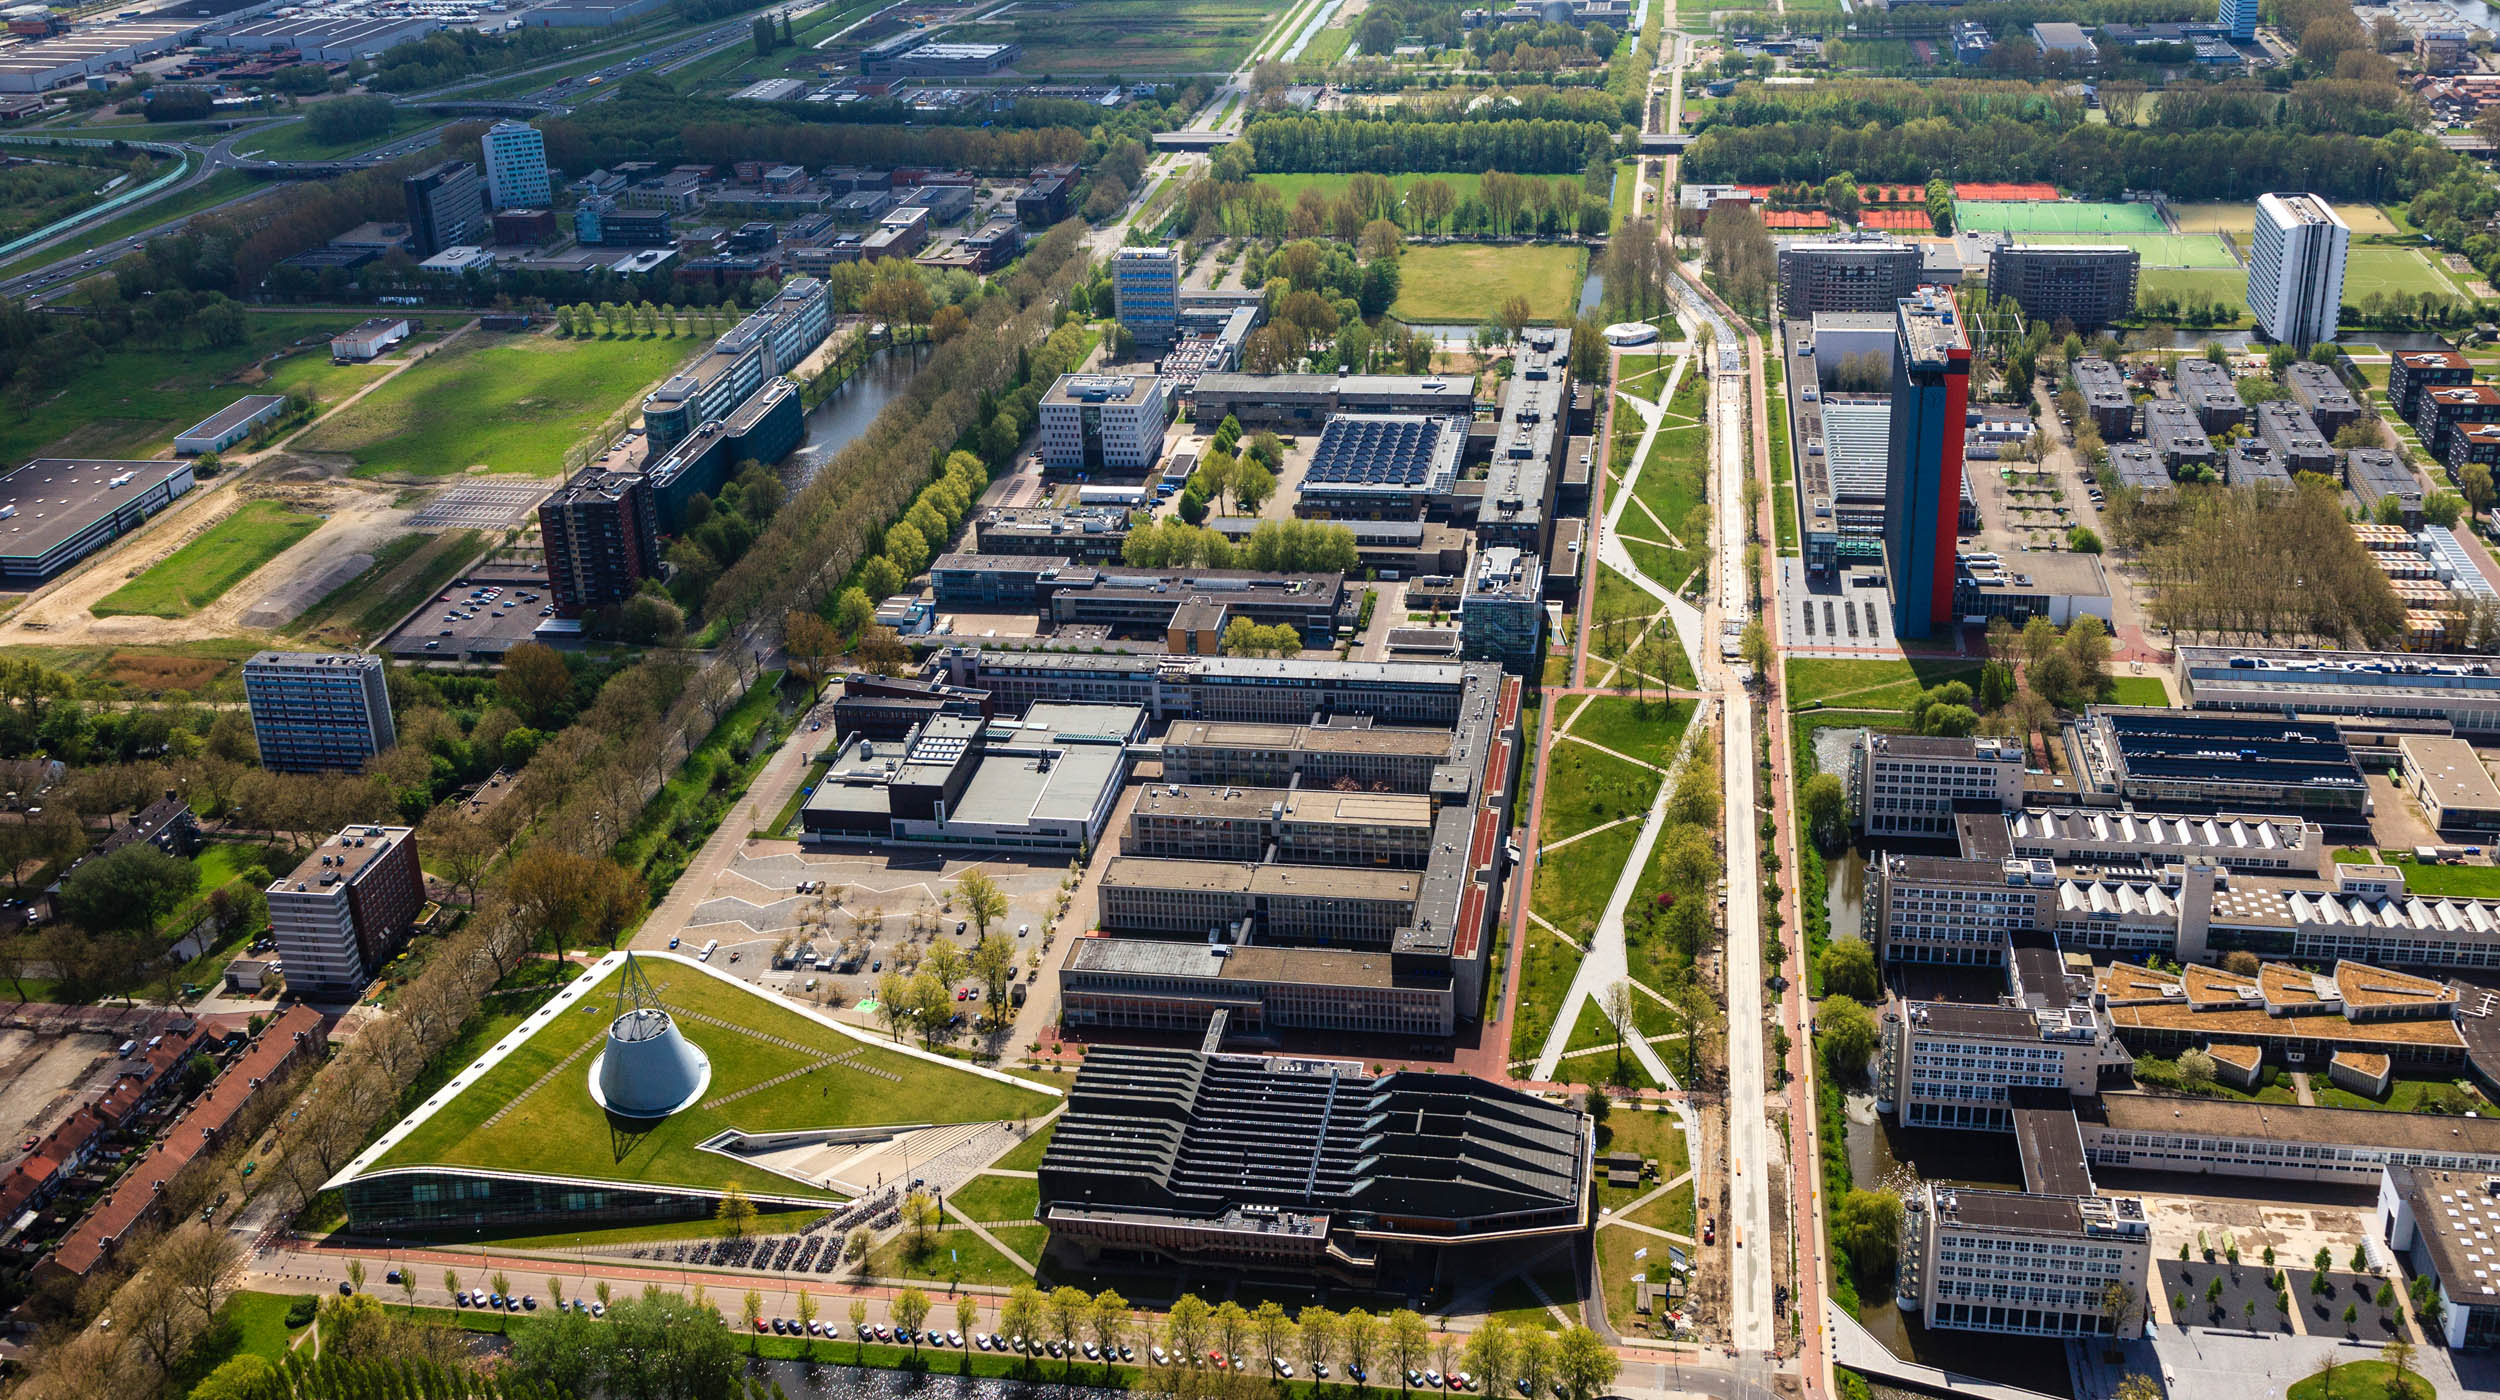
\includegraphics[width=1\textwidth]{images/aerial.jpg}
    \end{figure}
\end{frame}

\begin{frame}
    \delft
    \begin{figure}
        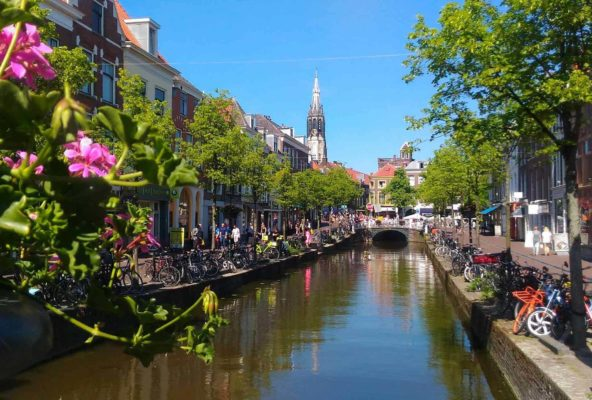
\includegraphics[width=0.9\textwidth]{images/beekje.jpg}
    \end{figure}
\end{frame}

\begin{frame}
    \delft
    \begin{figure}
        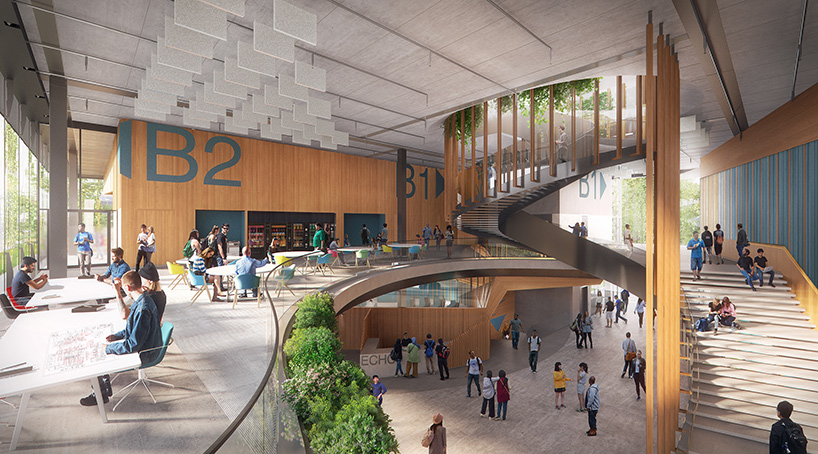
\includegraphics[width=0.9\textwidth]{images/echo.jpg}
    \end{figure}
\end{frame}

\begin{frame}
    \delft
    \begin{figure}
        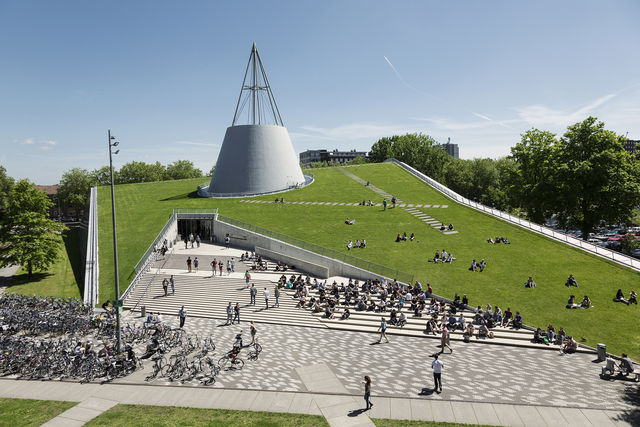
\includegraphics[width=0.9\textwidth]{images/library.jpg}
    \end{figure}
\end{frame}

\begin{frame}
    \delft
    \begin{figure}
        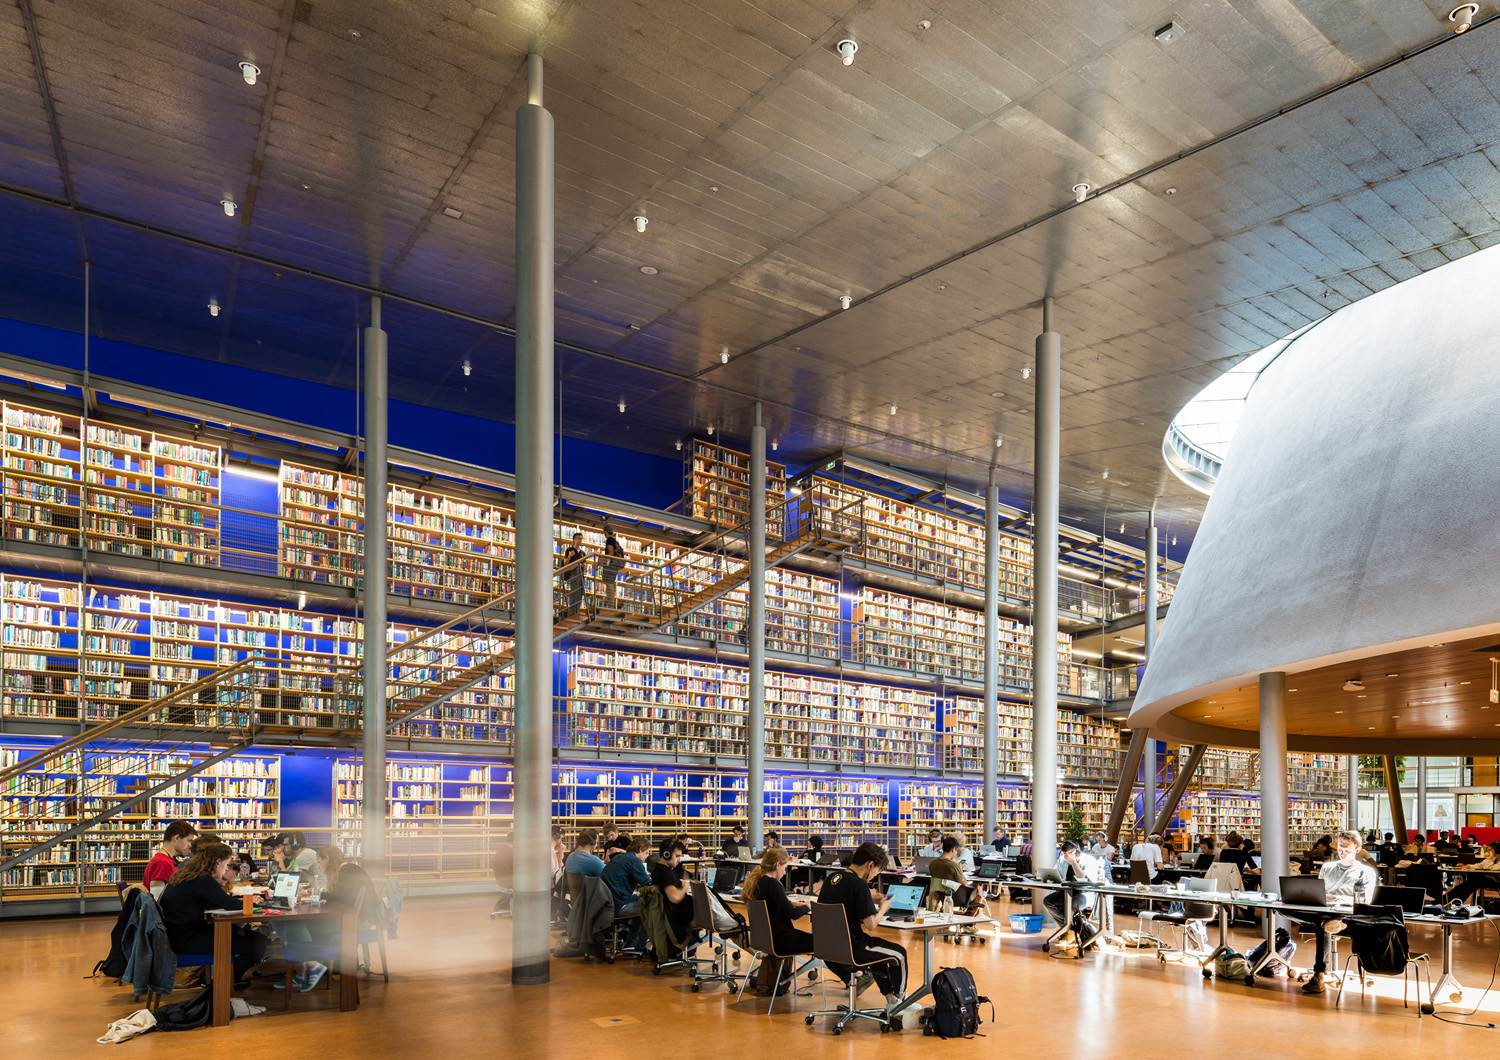
\includegraphics[width=0.9\textwidth]{images/books.jpg}
    \end{figure}
\end{frame}

\begin{frame}
    \delft
    \begin{figure}
        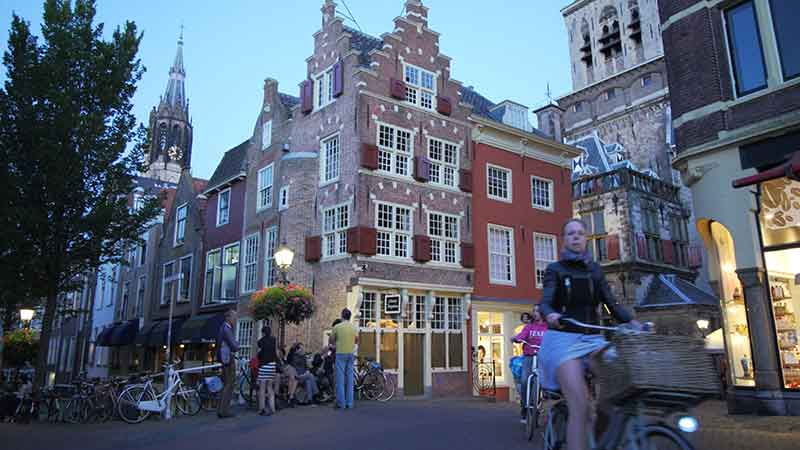
\includegraphics[width=0.9\textwidth]{images/delft-city.jpg}
    \end{figure}
\end{frame}

\begin{frame}
    \delft
    \begin{figure}
        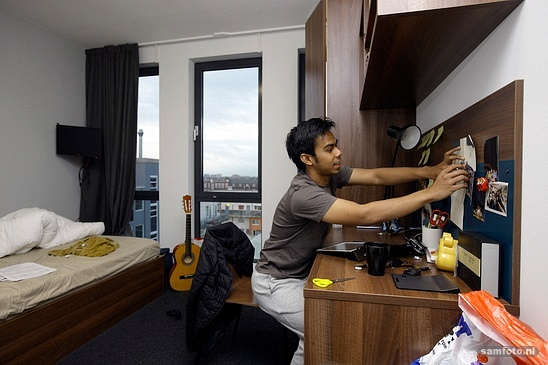
\includegraphics[width=0.9\textwidth]{images/duwo.jpg}
    \end{figure}
\end{frame}

\begin{frame}
    \delft
    \begin{figure}
        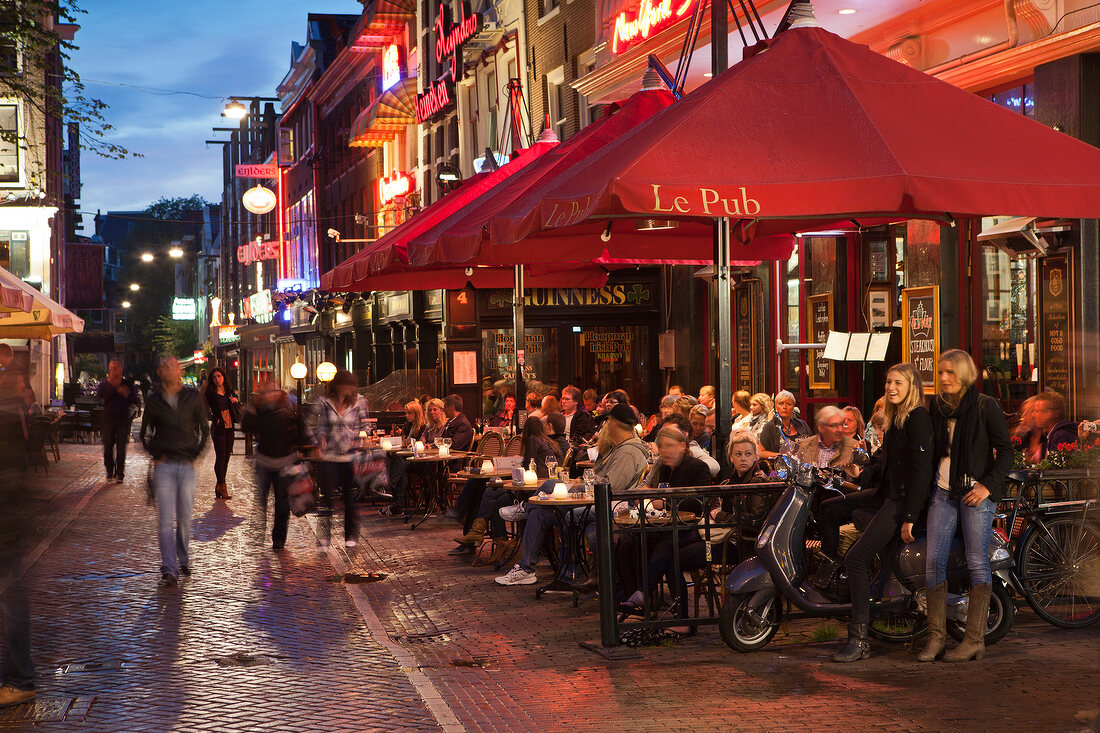
\includegraphics[width=0.9\textwidth]{images/lepub.jpg}
    \end{figure}
\end{frame}

\begin{frame}
    \delft
    \begin{figure}
        \centering
        \begin{tikzpicture}
            \node at (0,0) {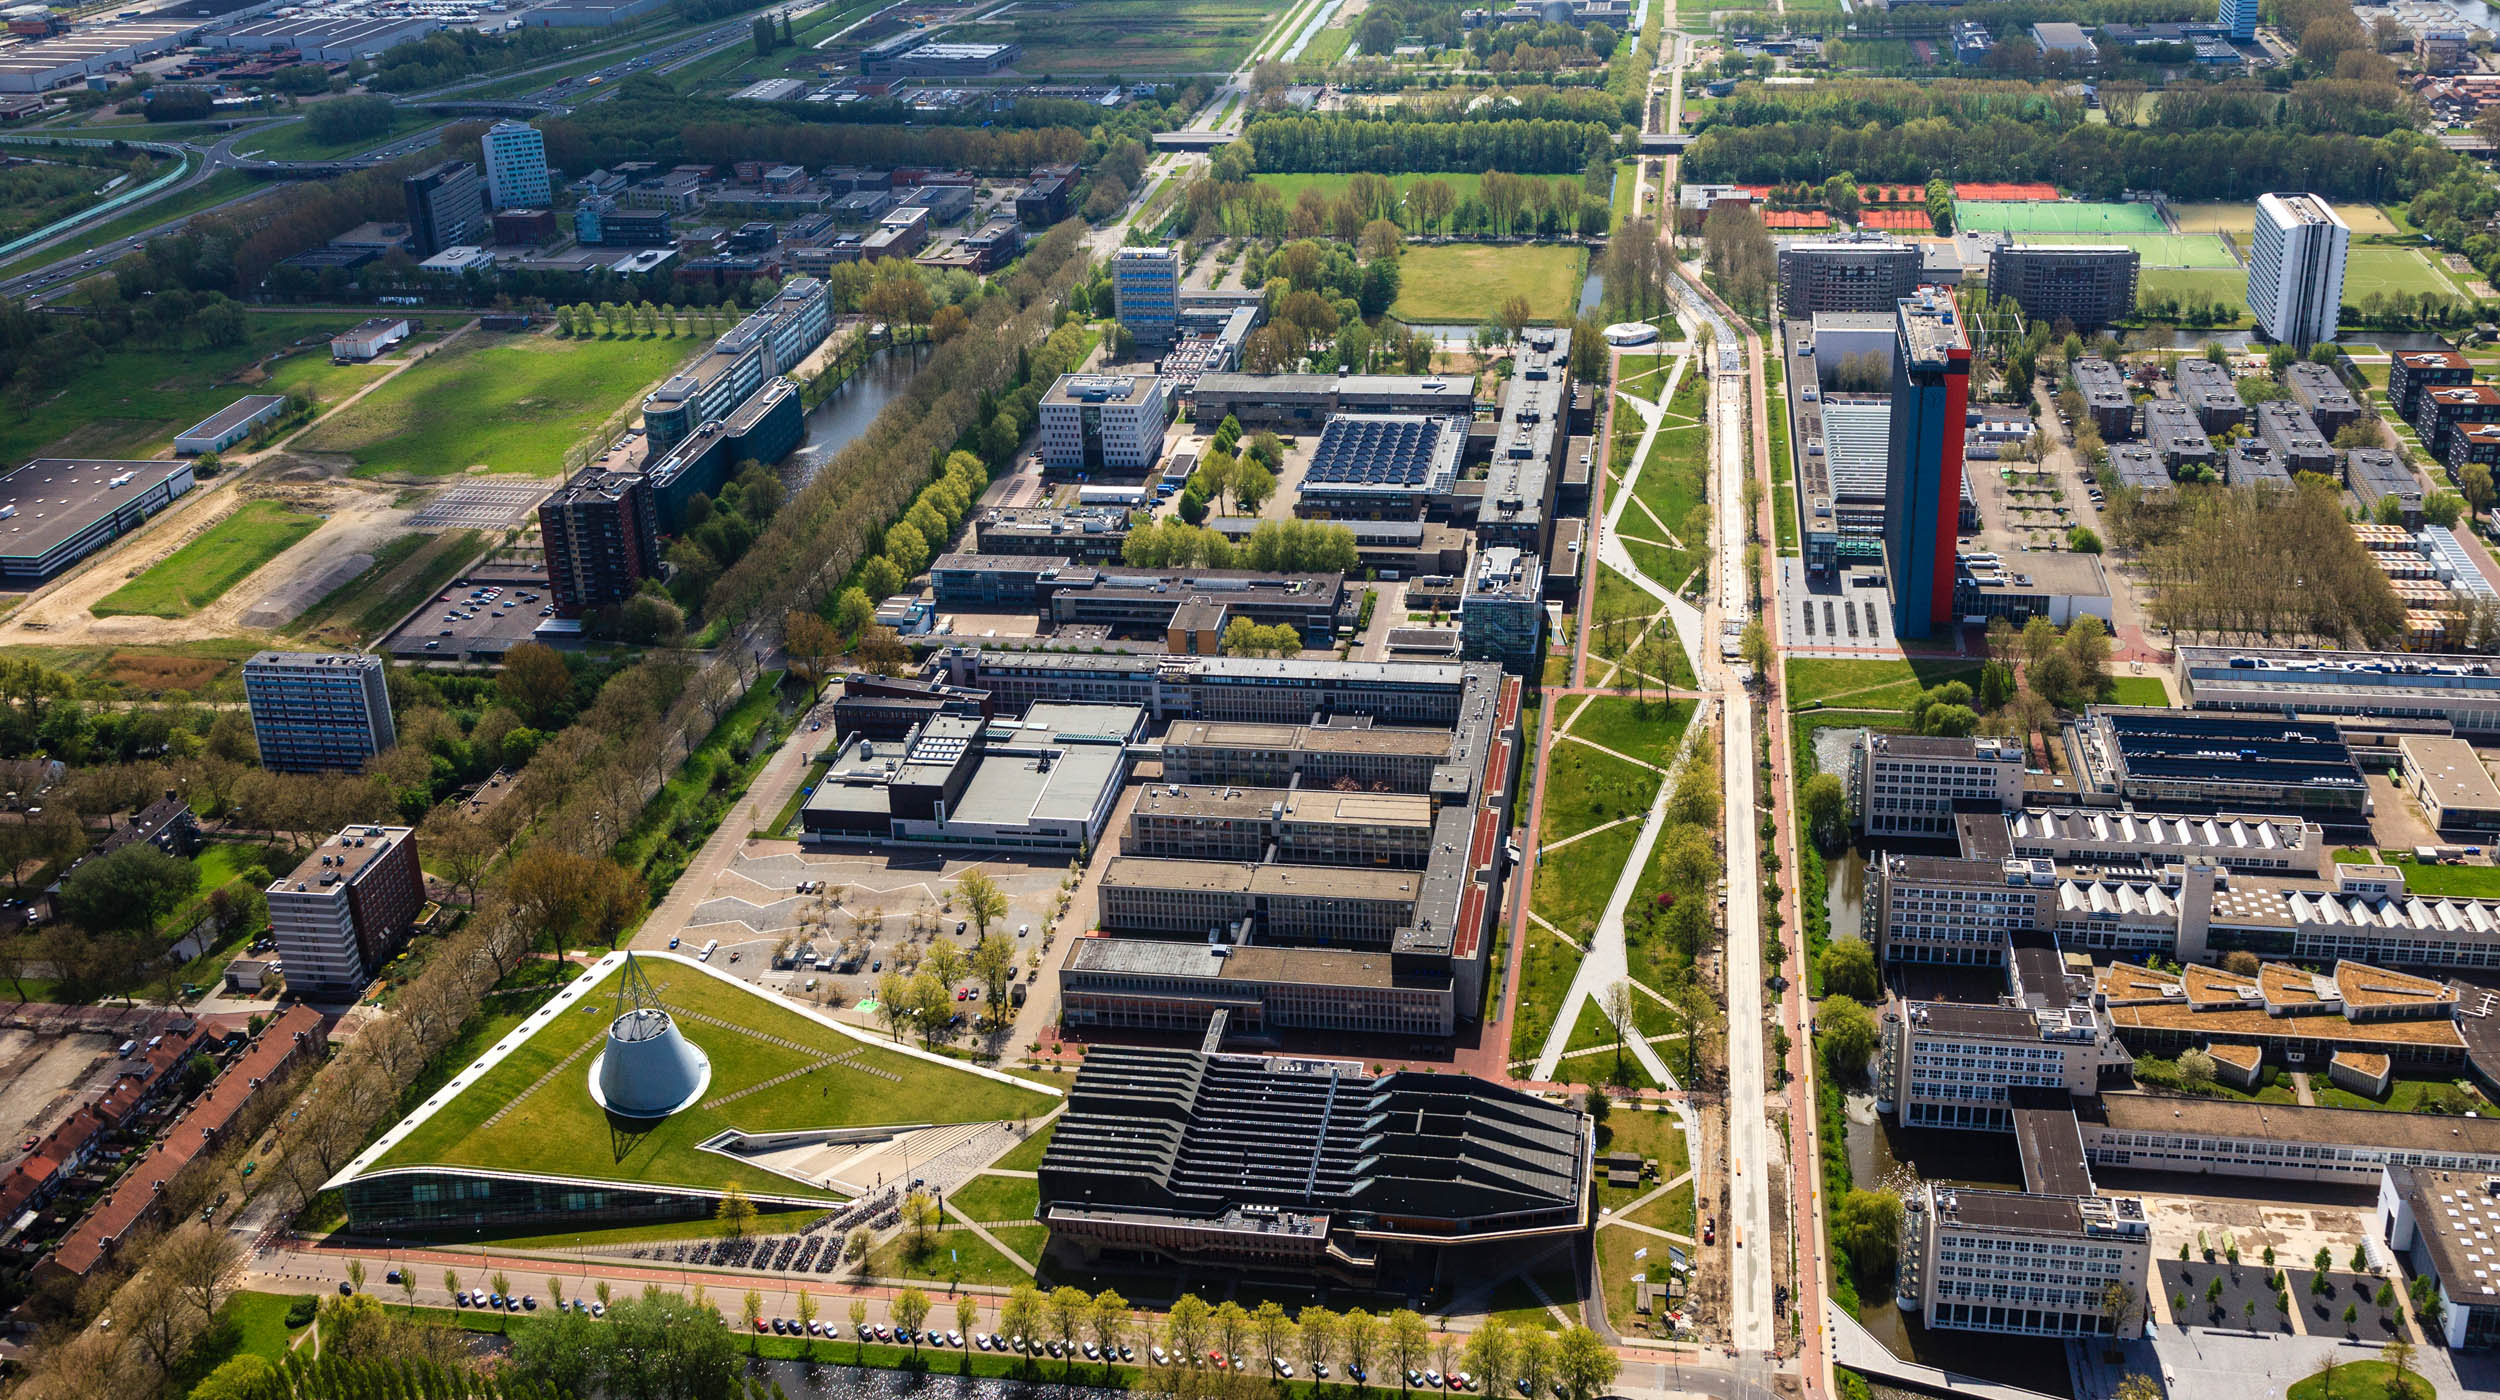
\includegraphics[width=0.9\textwidth]{images/aerial.jpg}};
            \node at (-3.7,-1.5) {
\includegraphics[width=0.3\textwidth]{images/qrcode.png }};
        \end{tikzpicture}
        \small https://www.tudelft.nl/onderwijs/toelating-en-aanmelding/exchange-students
    \end{figure}
\end{frame}



